\documentclass[10pt,a4paper]{article}
\usepackage[utf8]{inputenc}
\usepackage[francais]{babel}
\usepackage[T1]{fontenc}
\usepackage{hyperref}
\usepackage{eurosym}
\usepackage{ amssymb }
\usepackage{graphics}
\usepackage{pdfpages}
\usepackage{float}
\usepackage{amsmath}
\usepackage{amssymb}
\usepackage{fullpage}
\usepackage{blindtext}
\usepackage[section]{placeins}
\usepackage{color}
\usepackage{listings}


\def\ojoin{\setbox0=\hbox{$\bowtie$}%
  \rule[-.02ex]{.25em}{.4pt}\llap{\rule[\ht0]{.25em}{.4pt}}}
\def\leftouterjoin{\mathbin{\ojoin\mkern-5.8mu\bowtie}}
\def\rightouterjoin{\mathbin{\bowtie\mkern-5.8mu\ojoin}}
\def\fullouterjoin{\mathbin{\ojoin\mkern-5.8mu\bowtie\mkern-5.8mu\ojoin}}
\def\join{\bowtie}

\lstset{
  language=SQL,
  basicstyle=\ttfamily\footnotesize,        % the size of the fonts that are used for the code
  breakatwhitespace=false,         % sets if automatic breaks should only happen at whitespace
  breaklines=true,                 % sets automatic line breaking
  commentstyle=\color{cyan},    % comment style
  keepspaces=true,                 % keeps spaces in text, useful for keeping indentation of code (possibly needs columns=flexible)
  keywordstyle=\color{blue},       % keyword style
  numbers=left,                    % where to put the line-numbers; possible values are (none, left, right)
  numbersep=5pt,                   % how far the line-numbers are from the code
  numberstyle=\tiny\color{blue}, % the style that is used for the line-numbers
  rulecolor=\color{black},         % if not set, the frame-color may be changed on line-breaks within not-black text (e.g. comments (green here))
  showstringspaces=false,          % underline spaces within strings only
  showtabs=false,                  % show tabs within strings adding particular underscores
  stepnumber=5,                    % the step between two line-numbers. If it's 1, each line will be numbered
  stringstyle=\color{red},     % string literal style
  tabsize=2,                       % sets default tabsize to 2 spaces
}


\begin{document}

\begin{titlepage}
    \begin{center}
        \textbf{\textsc{UNIVERSIT\'E LIBRE DE BRUXELLES}}\\
        \vfill{}\vfill{}
        \begin{center}{\Huge Rapport : Annuaire d’établissements horeca}\end{center}{\Huge \par}
        \begin{center}{\large Romain \textsc{Fontaine}, Nikita \textsc{Marchant}}\end{center}{\Huge \par}
        \vfill{}\vfill{} \vfill{}
        \begin{flushleft}{\large \textbf{INFO-H-303 Base de données}}\hfill{Esteban Zimányi, Michaël Waumans}\end{flushleft}{\large\par}
        \vfill{}\vfill{}\enlargethispage{3cm}
        \textbf{Année académique 2015--2016}
    \end{center}
\end{titlepage}

\setlength{\parindent}{1.5em}
\setlength{\parskip}{1em}
\linespread{1.1}

\tableofcontents

\section{Diagramme entité association}
\subsection{Diagramme}
\begin{figure}[h]
    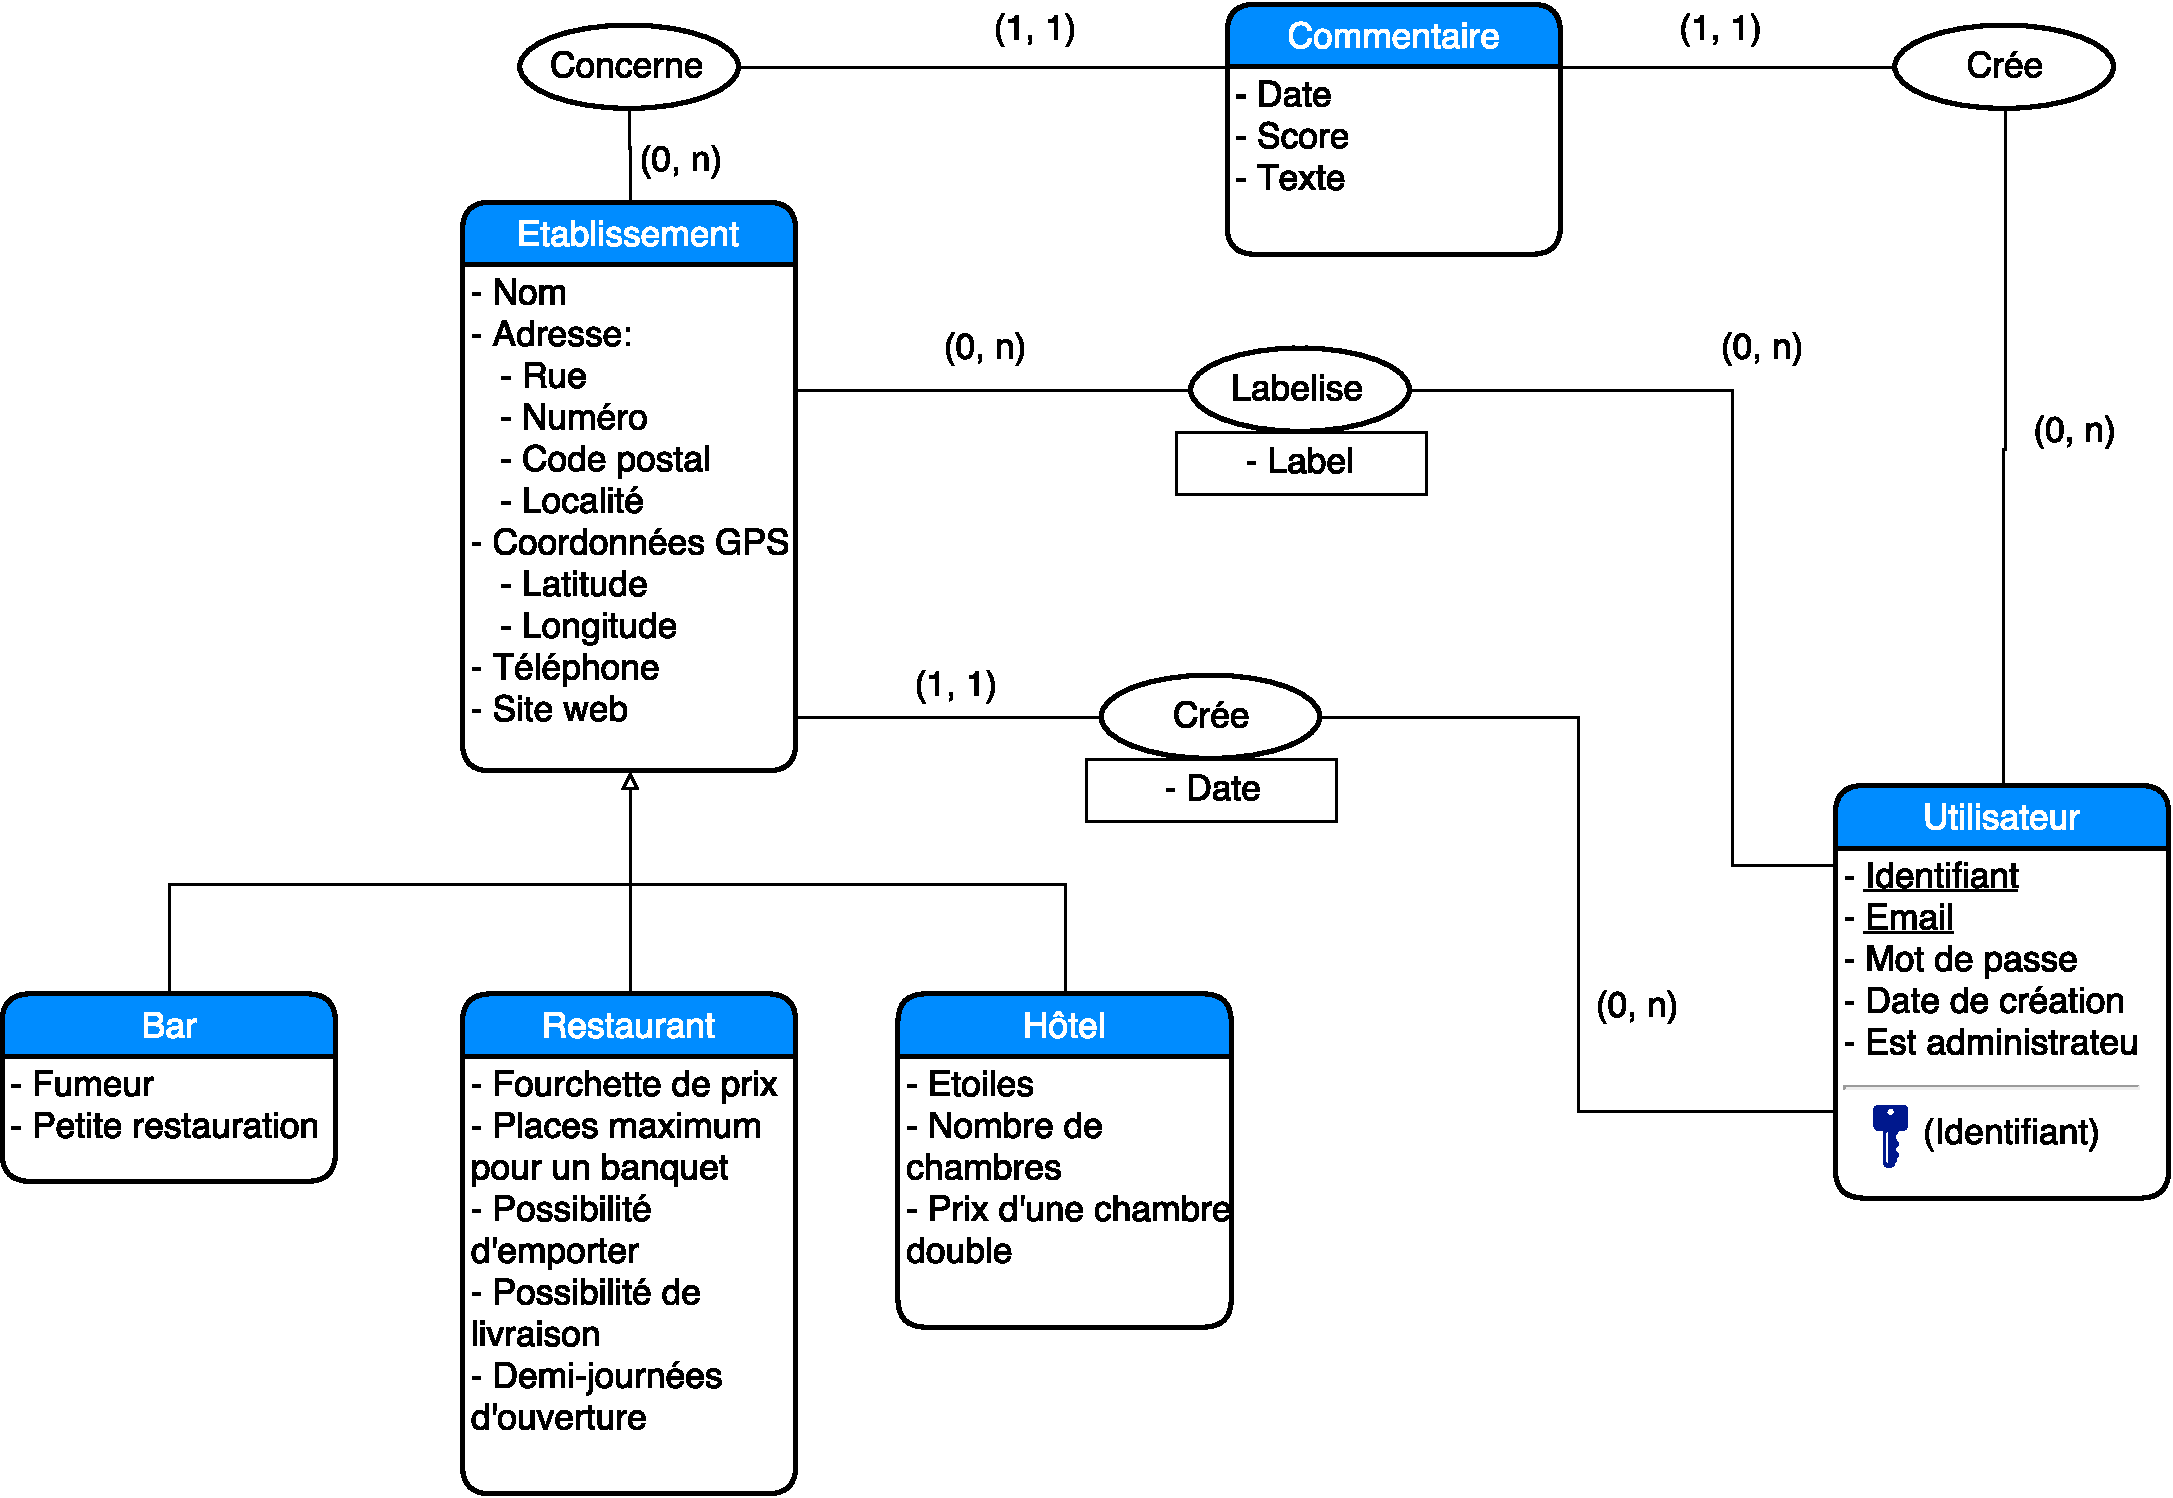
\includegraphics[scale=0.40]{EA.pdf}
    \caption{Diagramme Entité-Association}
    \label{diagram}
\end{figure}
\FloatBarrier

\subsection{Contraintes}

Les contraintes sont les suivantes :
\begin{itemize}
  \item L'\textit{UtilisateurId} d'un \textit{Etablissement} ne peut référencer qu'un \textit{Utilisateur} dont le champ \textit{EstAdministrateur} est vrai.
  \item La \textit{DateCretation} d'un \textit{Etablissement} doit être surpérieure à la \textit{DateCretation} de l'\textit{Utilisateur} qui l'a créé.
  \item La \textit{Latitude} (respectivement \textit{Longitude}) d'un \textit{Etablissement} doit appartenir à l'intervalte $[-90, 90]$ (respectivement $[-180, 180]$)
  \item Le champ \textit{Etoiles} d'un \textit{Hotel} doit appartenir à $[0,5]$
  \item Le champ \textit{Etoiles} d'un \textit{Commentaire} doit appartenir à $[0,5]$

\end{itemize}




\section{Modèle relationnel}
\subsection{Modèle}


\begin{description}
\item[Utilisateur](
    \underline{Id},
    \underline{Email},
    MotDePasse,
    DateCretaion,
    EstAdministrateur)

\item[Etablissement](
    \underline{Id},
    Type,
    Nom,
    Telephone,
    \textit{SiteWeb},
    Rue,
    Numero,
    CodePostal,
    Localite,
    Latitude,
    Longitude,
    DateCretation
    UtilisateurId)

    \begin{itemize}
        \item Etablissement.Type est une énumération de (Hotel, Bar, Restaurant)
        \item Etablissement.UtilisateurId référence Utilisateur.Id
    \end{itemize}

\item[Restaurant](
    \underline{EtablissementId},
    FourchettePrix,
    PlacesMaximum,
    Emporter,
    Livraison,
    DemiJoursOuverture)

    \begin{itemize}
        \item Restaurant.EtablissementId référence Etablissement.Id
    \end{itemize}

\item[Bar](
    \underline{EtablissementId},
    Fumeur,
    Restauration)

    \begin{itemize}
        \item Bar.EtablissementId référence Etablissement.Id
    \end{itemize}

\item[Hotel](
    \underline{EtablissementId},
    Etoiles,
    NombreChambres,
    PrixChambreDouble)

    \begin{itemize}
        \item Hotel.EtablissementId référence Etablissement.Id
    \end{itemize}

\item[Commentaire](
    \underline{Id},
    EtablissementId,
    UtilisateurId,
    Date,
    Score,
    Texte)

    \begin{itemize}
        \item Commentaire.EtablissementId référence Etablissement.Id
        \item Commentaire.UtilisateurId référence Utilisateur.Id
        \item (EtablissementId, UtilisateurId, Date) est unique
    \end{itemize}

\item[Label](
    \underline{Id},
    \underline{Nom})

\item[LabelEtablissement](
    \underline{Id},
    EtablissementId,
    UtilisateurId,
    LabelId)

    \begin{itemize}
        \item LabelEtablissement.EtablissementId référence Etablissement.Id
        \item LabelEtablissement.UtilisateurId référence Utilisateur.Id
        \item LabelEtablissement.LabelId référence Label.Id
        \item (EtablissementId, UtilisateurId, LabelId) est unique
    \end{itemize}

\end{description}

\section{Remarques}

Nous avons ajouté un champ \textit{Type} à la table \textit{Etablissement} pour pouvoir distinguer dans la table \textit{Etablissement} un bar d'un restaurant sans devoir \texttt{JOIN} sur les tables bar et restaurant. Cela nous permet par exemple de faire une requête ``Récupérer la liste des adresses des bars'' avec une simple \texttt{SELECT}.

De plus il faudra rajouter une contrainte pour que \textit{Bar.EtablissementId}, \textit{Restaurant.EtablissementId} et \textit{Hotel.EtablissementId} soient uniques, ce qui permet de garder la relation ``one-to-one'' entre \textit{Etablissement} et \textit{Bar}, \textit{Restaurant}, \textit{Hotel}.

Nous avons considéré que deux utilisateurs ne peuvent avoir la même adresse email; l'adresse email d'un \textit{Utilisateur} doit donc être unique.


\section{Sript DDL de création de la base de données}
\lstinputlisting{../flask/createdb.sql}

\section{Requêtes}

\section{R1}
\subsection{AR:}
\(
BC(C_1, C_2, C_3) \leftarrow \pi_{C_1.eid, C_2.eid, C_3.eid} (((C_1 \join_{C_1.id != C_2.id \land C_1.score > 3 \land C_2.score>3} C_2)\\
\join_{C_1.id != C_3.id \land C_2.id != C3.id \land C_3.score>3}) \join_{C_1.uid = U.id \land C_2.uid = U.id \land C_3.uid = U.id}(\sigma_{U.username = "Brenda"}(U)))
\)\\

\(
AC(uid, C_1, C_2, C_3) \leftarrow \pi_{U.id, C_1.eid, C_2.eid, C_3.eid} (((C_1 \join_{C_1.id != C_2.id \land C_1.score > 3 \land C_2.score>3} C_2)\\
\join_{C_1.id != C_3.id \land C_2.id != C3.id \land C_3.score>3}) \join_{C_1.uid != U.id \land C_2.uid != U.id \land C_3.uid != U.id}(\sigma_{U.username = "Brenda"}(U)))
\)\\

\(
\pi_{AC.uid}(BC \join_{BC.C_1 = AC.C_1 \land BC.C_2 = AC.C_2 \land BC.C_3 = AC.C_3} AC)
\)

\subsection{TC}
\(
\{
u|users(u) \land \exists b(users(b) \land b.username="Brenda") \land u.id \neq b.id
\land\\
\exists e_1(etablissement(e_1) \land \exists c_1 \exists c_2(comment(c_1)\land comment(c_2) \land c_1.uid = u.id \land c_1.score > 3 \land c_2.uid = b.uid \land c_2.score >3))
\land\\
\exists e_2(etablissement(e_2) \land e_1 \neq e_2 \land \exists c_3 \exists c_4(comment(c_3)\land comment(c_4) \land c_3.uid = u.id \land c_3.score > 3 \land c_4.uid = b.uid \land c_4.score >3))
\land\\
\exists e_3(etablissement(e_3) \land e_1 \neq e_3 \land e_2 \neq e_3 \land \exists c_5 \exists c_6(comment(c_5)\land comment(c_6) \land c_5.uid = u.id \land c_5.score > 3 \land c_6.uid = b.uid \land c_6.score >3))
\}
\)

\section{R2}
\subsection{AR}
\(
AC \leftarrow \pi_{C.uid, C.eid}(\sigma_{C.score>3}(C))
\\
BC \leftarrow \pi_{C.eid}(\sigma_{U.name="Brenda", C.score>3}(C*U))
\\
U \leftarrow  \pi_{AC.uid}(AC \div BC)
\\
\pi_{C.eid}(\sigma_{C.uid = U.uid \land C.score>3}(C))
\)

\subsection{TC}
\(
\{
e|etablissement(e) \land \exists c(comment(c) \land c.score>3 \land c.eid = e.id \land \exists u(users(u) \land c.uid = u.id \land \forall f \forall b(comment(f) \land users(b) \land f.uid = b.uid\land b.username="Brenda" \land f.score > 3 \rightarrow \exists a(comment(a)\land a.uid = u.id \land f.eid = a.eid\land a.score > 3)))))
\}
\)

\section{R3}
\subsection{AR}
\(
Ew2C \leftarrow \pi_{C_1.eid, C_1.id}(C_1 \join_{C_1.eid=C_2.eid \land C_1.id != C_2.id})
\\
\pi_{E.id}(\pi_{E.id, C.id}(E \leftouterjoin_{E.id=C.eid}  C) - EW2C)
\)
\subsection{TC}

\(
\{e | etablissement(e) \land \exists c(comment(c) \land c.eid = e.id) \rightarrow \neg\exists d(comment(d) \land d.eid = e.id \land d.id \neq c.id)\}
\)

\section{R4}
\subsection{AR}
\(
\pi_{E.uid}(E) - \pi_{E.id}(E\join_{E.id = C.id \land E.uid = C.uid}C)
\)
\subsection{TC}
\(
\{e.uid|etablissement(e)\land \neg \exists c(comment(c) \land c.uid = e.uid \land c.eid = e.id)\}
\)


\section{Implémentation et choix}

Le projet peut être exécuté en suivant les instructions se trouvant dans le fichier readme à la racine du projet.

\subsection{Language et bibliothèques}

Nous avons choisi d'utiliser \textbf{Python 3} ainsi que le framework \textbf{Flask} pour implémenter notre application web. Nous avons choisi \textbf{Python 3} car il est notre langage de prédilection et qu'il dispose d'un écosystème de librairies très développé.

Nous nous étions d'abord tourné vers \textbf{Django} pour le framework web car nous avons tous les deux de l'expérience avec celui-ci et qu'il est très puissant pour prototyper rapidement (gestion automatique du CRUD\footnote{CReate, Update, Delete}, validation des formulaires, gestion des utilisateurs incluse, ...) mais après avoir rapidement essayé de l'utiliser dans utiliser son \textit{ORM} (qui fait aussi \textit{query-builder}) pour suivre les consignes, nous nous somme rendus compte que nous perdions touts les avantages de \textbf{Django} tout en gardant ses inconvénients.

Nous nous sommes donc tournés vers le framework \textbf{Flask}, qui est beaucoup plus minimal et qui nous a donc laissé plus libres dans nos choix d'implémentation, celui-ci ne proposant ni d'ORM, ni de gestion des utilisateurs ni de validation de formulaires.

Pour l'interface utilisateur, côté serveur, nous avons utilisé le moteur de template \textbf{Jinja2} qui vient directement avec \textbf{Flask}, la librairie de validation \textbf{WTF-Forms}. Côté client, nous avons utilisé \textbf{Bootstrap3} pour la base du CSS et \textbf{Leaflet} pour l'affichage des cartes.

\subsection{Base de donnée}

Nous avons rapidement écarté \textbf{SQLite} car celui-ci ne permet pas d'accès concurrents.

Notre choix s'est porté sur \textbf{Postgresql} plutôt que \textbf{MySQL} car le premier est un des moteurs les plus complets, puissants et rapides du marché. De plus, il permet, contrairement à MySQL, d'ajouter des contraintes et il supporte les \textit{ARRAY}.

\subsubsection{Contraintes}

Nous n'avons pas implémenté les contraintes nécessitent de vérifier plusieurs tables à la fois (comme par exemple: ``la date de création d'un établissement doit être supérieure à celle d'inscription de l'utilisateur qui le crée'') car \textbf{Postgresql} (\textbf{MySQL}, \textbf{SQLite}) ne le permet pas à l'aide du mot clé \texttt{CHECK}.

Nous nous sommes documentés et il semblerait qu'il soit possible de déclarer des \texttt{TRIGGER} qui sont déclenchés à l'insertion d'une ligne et dans lequel il est possible de faire tourner plus de logique mais ils nous a semblé qu'implémenter cette solution était hors du cadre de ce projet.

\subsubsection{Indexes}



\subsubsection{\texttt{ON DELETE}}

Nous avons décidé que les suppressions dans la base de donnée devraient résulter en la suppression des entités liées (\texttt{ON DELETE CASCADE}) car par exemple, il nous semble logique qu'il ne faut pas garder un commentaire si l'établissement sur lequel il porte n'existe plus.

La seule entorse à cette règle a été pour les administrateurs. Si un administrateur ne peut être supprimé si il a des établissements (\texttt{ON DELETE RESTRICT}).

\subsection{Script d'insertion des données}

\subsection{Modèles}

Nous avons écrit un ORM minimal pour simplifier l'insertion, la mise à jour ainsi que le mapping résultat---objet.

Pour cela, chaque modèle définit une liste de champs à sélectionner dans la base de donnée, la liste des champs en auto-increment (pour ne pas essayer de les définir à l'insertion) ainsi que les foreign-keys.

La spécification des foreign-keys nous permet, lors de jointures de faire automatiquement le mapping pour les objets liés.

L'ORM nous aide aussi à écrire des requêtes avec deux méthodes : la première est lors du \texttt{SELECT}, \texttt{Model.star()} renvoie la liste des champs préfixées par le nom de la table pour que nous n'ayons pas à l'écrire à chaque fois. La seconde est utile lors des \texttt{INSERT} et \texttt{UPDATE} et permet de spécifier toutes les colonnes utiles et nous permet aussi de ne pas devoir l'écrire à chaque fois.

Le reste des requêtes apparaît en clair dans le code.

\section{Apports personnels}

\subsection{Intégration de Leaflet}

Pour rendre l’interaction avec notre application plus visuelle nous avons ajouté des cartes à plusieurs endroits. Celles-ci sont affichées grâce à Leaflet, une bibliothèque Javascript libre et utilisent des fonds de carte OpenSreetMap.

Nous affichons par exemple une carte avec tous les établissements sur la page d'accueil et nous la centrons sur la position courante de l'utilisateur (récupérée en Javascript) pour rendre l'accueil plus personnalisé.

Une carte est aussi affichée lors d'une recherche et permet de visualiser rapidement les différents résultats.

Pour finir, chaque page d'un établissement situe celui-ci sur une petite carte.

\subsection{Interface responsive et mobile friendly}

L'utilisation d'internet étant de plus en plus mobile, nous avons développé notre interface web en faisant attention que celle-ci soit facilement utilisable sur des terminaux mobiles grâce à une interface responsive qui s'adapte autant aux grands écrans de PC qu'à des petits smartphones an passant par des tablettes.

\subsection{Design}

Nous avons fait plus que simplement utiliser \textbf{Bootsrap} pour notre interface : nous avons écrit une série de règles css pour rendre notre site web moins générique et plus attrayant. Petite touche humoristique, nous nous sommes inspirés de la charte graphique du site \textit{Foursquare}, d'ou le nom de notre application : \textit{FourTriangle}.

\subsection{Images}

Chaque établissement dispose d'une photo qui peut être uploadée par les administrateurs. Celle-ci est affichée dans la liste des établissement ainsi que sous forme de bannière sur la page de l'établissement même.

De plus, les utilisateurs ont aussi une photo sur leur profil. Pour cela, nous utilisons le service \textit{Gravatar} qui permet aux utilisateurs de définir leur photo de profil une seule fois et qu'elle apparaisse sur tous les sites web à la fois.

\subsection{Recherche \textit{fuzzy}}

La recherche d'établissement est effectuée sur le champ ``nom'' mais n'attend pas une correspondance exacte (comme un \texttt{WHERE ==} ou un \texttt{LIKE}) mais effectue une recherche basée sur la similarité entre les deux chaînes. Ceci permet à l'utilisateur de faire des fautes d'orthographe et de quand même trouver ce qu'il cherche.

De plus, si un seul résultat est trouvé, l'utilisateur est directement redirigé sur celui-ci.

\subsection{CRUD pour tous les modèles}

Tous les modèles sont éditables et supprimables par l'utilisateur auxquels ils appartiennent ou par les administrateurs :

\begin{itemize}
    \item Un tag peut être édité, ajouté ou supprimé par un administrateur
    \item Un utilisateur peut changer ses informations et son mot de passe
    \item Un administrateur peut éditer tous les utilisateurs
    \item Un administrateur peut promouvoir ou dégrader d'autres administrateurs.
    \item Les établissements peuvent être crées, modifiés ou supprimés par des administrateurs
    \item Des commentaires peuvent être ajoutés
    \item Les commentaires peuvent être supprimés et édités par leur propriétaire ainsi que les administrateurs
\end{itemize}

\subsection{Sécurité}

Les mots de passe des utilisateurs sont hashés et salés avec la fonction cryptographique \textit{pbkdf2}. Celle-ci est réputée pour sa robustesse et sa complexité élevée d'attaque.

De plus, toutes les actions sont contrôlées du côté serveur, que ce soit pour vérifier leur validité (par exemple que l'adresse mail est valide) ou pour vérifier que l'utilisateur courant a bien le droit d'effectuer cette action.

\subsection{Validation côté client}

Les formulaires sont aussi validés du côté client ce qui permet à l'utilisateur d'avoir un retour dynamique en direct sur ses entrés plutôt que de soumettre un formulaire et de recevoir une erreur en retour si celui-ci est invalide.

\section{Annexe : captures d'écran}
\begin{center}
\begin{figure}[H]
   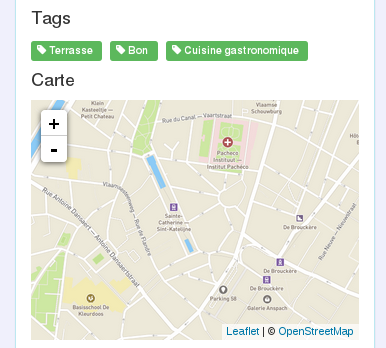
\includegraphics[width=5cm]{screen/carte.png}
   \caption{Carte sur un établissement}
\end{figure}


\begin{figure}[H]
   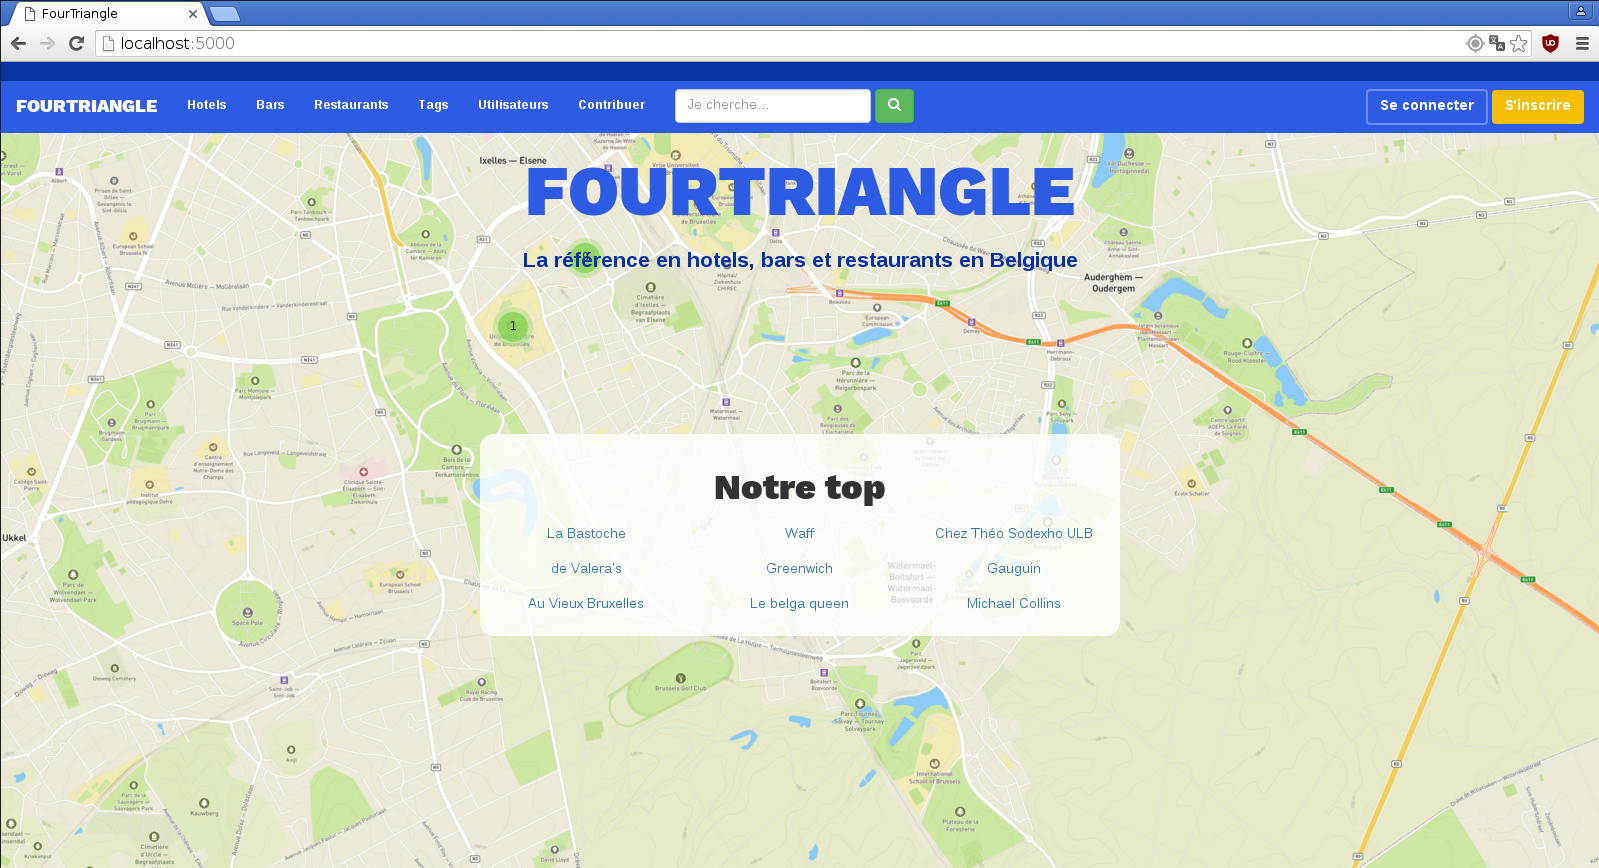
\includegraphics[width=15cm]{screen/home.png}
   \caption{Page d'accueil}
\end{figure}


\begin{figure}[H]
   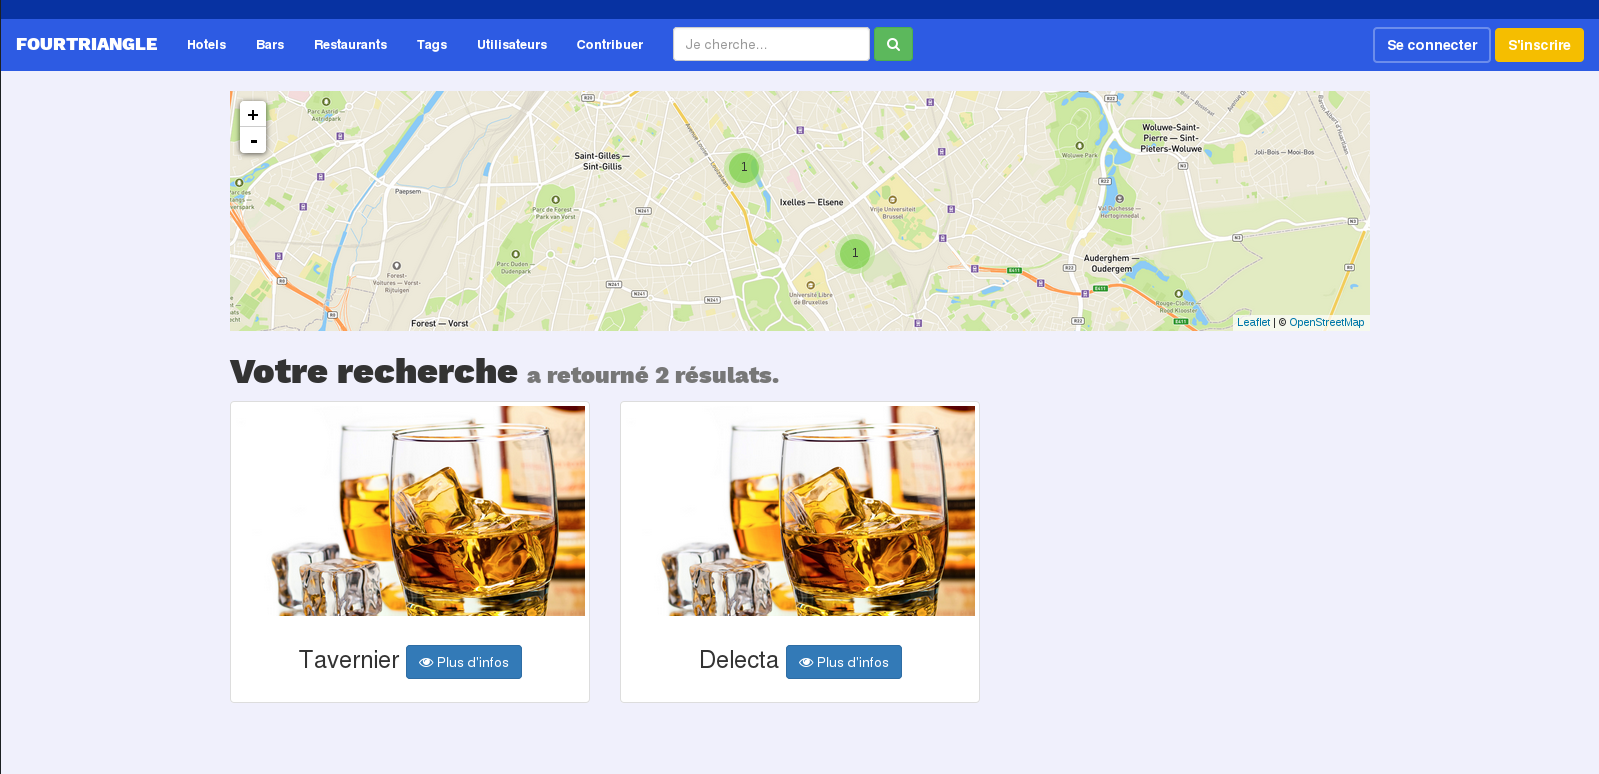
\includegraphics[width=15cm]{screen/recherche.png}
   \caption{Recherche}
\end{figure}


\begin{figure}[H]
   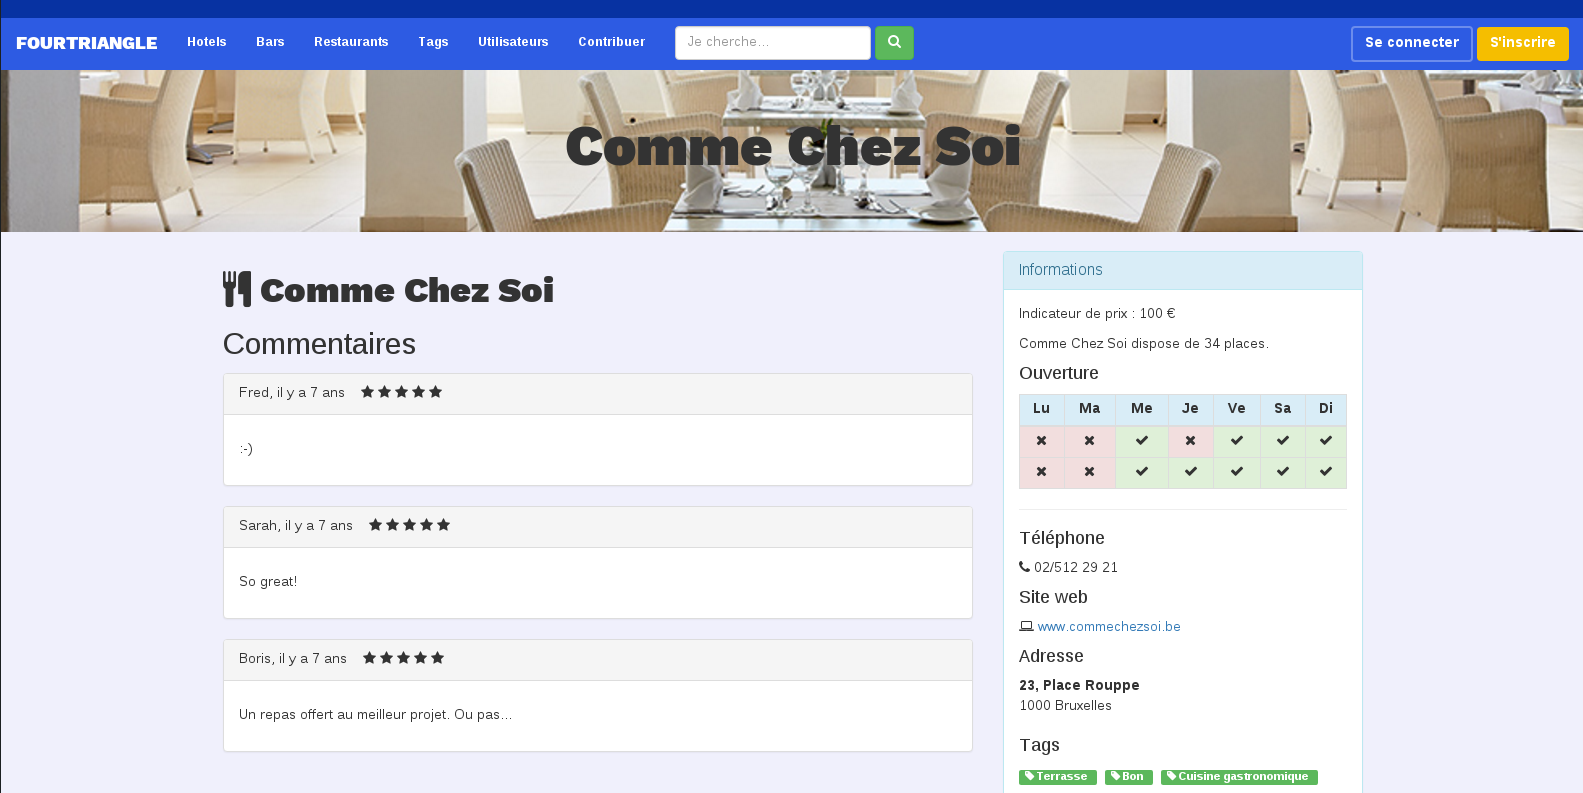
\includegraphics[width=15cm]{screen/resto.png}
   \caption{Vue d'un restaurant}
\end{figure}


\begin{figure}[H]
   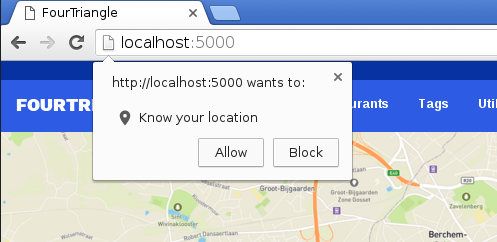
\includegraphics[width=15cm]{screen/geoloc.png}
   \caption{Géo-localistaion}
\end{figure}


\begin{figure}[H]
   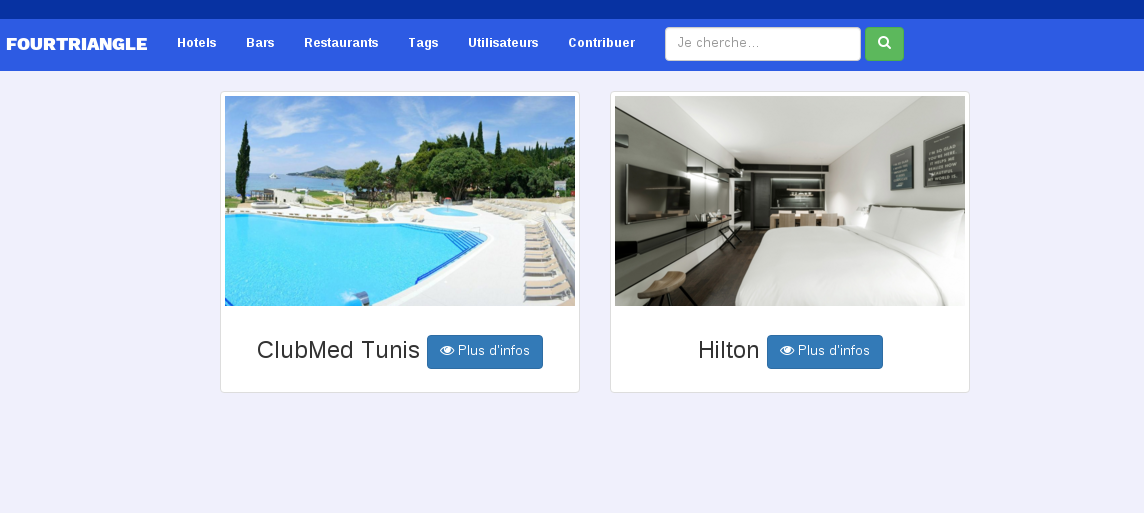
\includegraphics[width=15cm]{screen/list.png}
   \caption{Liste des hotels}
\end{figure}


\begin{figure}[H]
   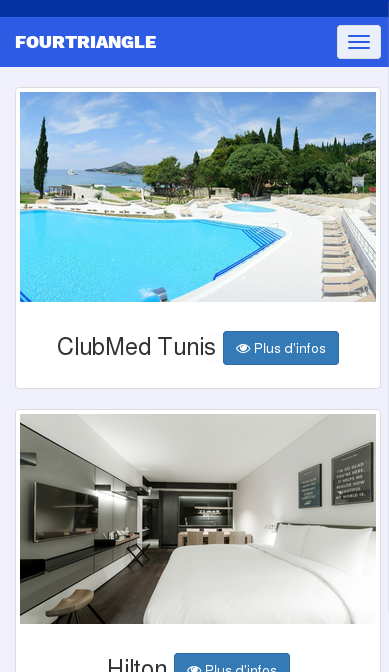
\includegraphics[width=5cm]{screen/responsive.png}
   \caption{Interface mobile}
\end{figure}


\begin{figure}[H]
   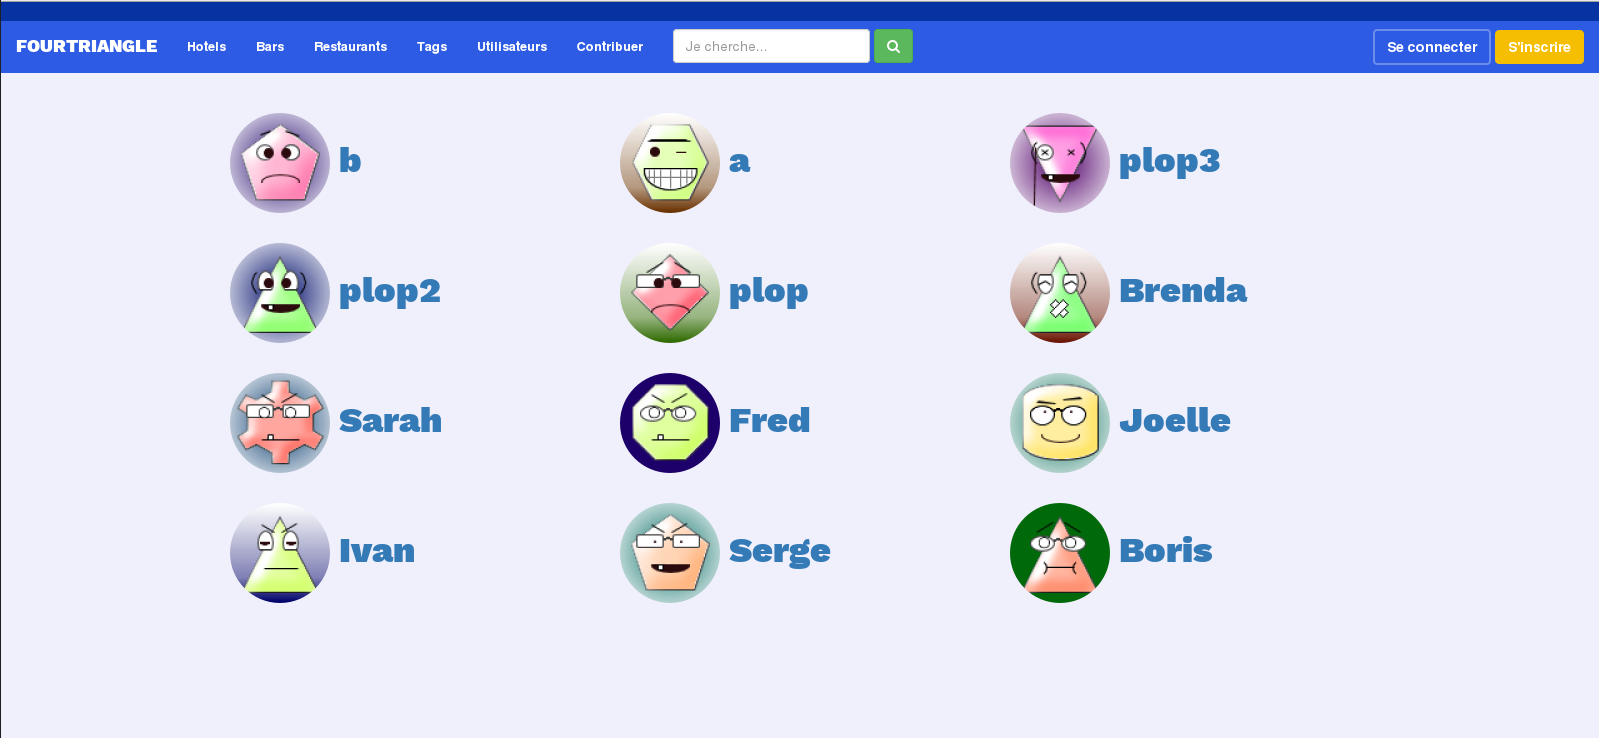
\includegraphics[width=15cm]{screen/users.png}
   \caption{Liste des utilisateurs}
\end{figure}
\end{center}
\end{document}

